\documentclass[12pt]{article}
\usepackage{ctex}

\usepackage[top=.8in, bottom=.8in, left=.8in, right=.8in]{geometry}
\usepackage{amsmath}
\usepackage{tikz}
\usetikzlibrary[topaths]
\newcount\mycount
\usepackage{amssymb,latexsym}
\usepackage{amsxtra}
\usepackage{amsthm}
\usepackage{graphicx}
\usepackage{setspace}
\onehalfspacing
\usepackage{wasysym} 
\usepackage{verbatim} 
\usepackage{arcs}
\usepackage{accents}
\theoremstyle{definition}
\usepackage[skins]{tcolorbox}
\tcbuselibrary{skins,theorems}
\tcbuselibrary{breakable}
%---------------------- New-environment ----------------
\newenvironment{Proof}
{
\vspace{-0.5cm}
\paragraph{\textcolor[rgb]{0.1,0.8,0.9}{\textsf{Proof}}}
}
{\hfill$\square$\vspace{0.3cm}}

\newenvironment{Remark}
{
\paragraph{\textcolor[rgb]{0.9,0.0,0.6}{\textsf{Remark}}}
}

%----------------------

\usepackage{hyperref}
\hypersetup{
    colorlinks=true,
    linkcolor=black,
    filecolor=magenta,      
    urlcolor=cyan,
    pdftitle={Overleaf Example},
    pdfpagemode=FullScreen,
    }
\urlstyle{same}


%-----------------------------------------------------------------------------%
\newtheorem{definition}{Definition}[section]
\newtheorem{example}{Example}[section]
\newtheorem{theorem}{Theorem}[section]
\newtheorem{proposition}{Proposition}[section]
\newtheorem*{fact}{Fact}
\newtheorem{remark}{Remark}
\newtheorem{corollary}{Corollary}[section]
\newtheorem{lemma}{Lemma}[section]


\newcommand{\df}{\displaystyle \frac} 
\newcommand{\dlim}{\displaystyle \lim}
\newcommand{\dint}{\displaystyle \int}
\newcommand{\ra}{\rangle}
\newcommand{\la}{\langle}
\newcommand{\inner}[2]{{\langle #1,#2\rangle}}
\newcommand{\x}{\mathbf{x}}
\newcommand{\xt}{\mathbf{x}^{\mathsf{T}}}
\newcommand{\T}{{\mathsf{T}}}
\newcommand{\abf}{\mathbf{a}}
\newcommand{\abft}{\mathbf{a}^{\mathsf{T}}}
\newcommand{\R}{\mathbb{R}}
\newcommand{\C}{\mathbb{C}}
\newcommand{\E}{\mathrm{e}}
\newcommand{\F}{\mathbb{F}}
\newcommand{\X}{\mathbf{X}}
\newcommand{\Y}{\mathbf{Y}}
\newcommand{\f}{\mathbf{f}}
\newcommand{\U}{\mathbf{u}}
\newcommand{\D}{\mathrm{d}}
\newcommand{\MCG}{\mathcal{G}}
\newcommand{\MCF}{\mathcal{F}}
\newcommand{\M}{\mathcal{M}}
\newcommand{\MCB}{\mathcal{B}}
\newcommand{\MCT}{\mathcal{T}}
\newcommand{\LL}{\mathcal{L}}
\newcommand{\nullspace}{\mathrm{null}}
\newcommand{\range}{\mathrm{range}}
\newcommand{\Sum}[2]{{\sum_{#1}^{#2}}}
\newcommand{\Union}[2]{{\bigcup_{#1}^{#2}}}
\newcommand{\Intersection}[2]{{\bigcap_{#1}^{#2}}}


\newcommand{\pd}[1]{\frac{\partial}{\partial #1}}
\definecolor{my-violet}{rgb}{0.9,0.0,0.6}

\newtcbtheorem[auto counter,number within=section]{stheorem}{Theorem}
{
	breakable,
	fonttitle=\bfseries\upshape,description font=\bfseries\itshape,
	arc=3mm, ,separator sign = \ ,
	theorem number and name,
	colbacktitle=blue!25!white,colback=blue!8!white,colframe=black,coltitle=black,
	toptitle=1.5mm,bottomtitle=1.5mm, 
}{th}

\newtcbtheorem[use counter from=stheorem]{sdefinition}%
  {定义}{breakable,fonttitle=\bfseries\upshape,description font=\bfseries\itshape,
     arc=3mm, ,separator sign = \ ,
     theorem number and name,
     colbacktitle=yellow!50!white,colback=yellow!15!white,colframe=black,coltitle=black,
     toptitle=1.5mm,bottomtitle=1.5mm,
     }{def}
     
\newtcbtheorem[use counter from=stheorem]{sconclude}%
  {}{breakable,fonttitle=\bfseries\upshape,description font=\bfseries\itshape,
     arc=3mm, ,separator sign = \ ,
     theorem number and name,
     colbacktitle=yellow!50!white,colback=yellow!15!white,colframe=black,coltitle=black,
     toptitle=1.5mm,bottomtitle=1.5mm,
     }{def}

\newtcbtheorem[use counter from=stheorem]{scorollary}%
  {定理}{breakable,fonttitle=\bfseries\upshape,description font=\bfseries\itshape,
     arc=3mm, ,separator sign = \ ,
     theorem number and name,
     colbacktitle=blue!25!white,colback=blue!8!white,colframe=black,coltitle=black,
     toptitle=1.5mm,bottomtitle=1.5mm,
     }{cr}
     
\newtcbtheorem[use counter from=stheorem]{sexample}%
  {Example}{breakable,theorem style=plain,separator sign = \ ,
  	fonttitle=\sffamily\normalsize,description font=\sf\itshape,
  	colbacktitle=black!11!white,coltitle=black,colframe=black,
    arc=0mm,outer arc=0mm,
    toptitle=1.5mm,bottomtitle=1.5mm,left=1mm,right=1mm,
	boxrule=0mm,toprule=0.5mm,bottomrule=.5mm,	rightrule=0mm,titlerule=0mm,top=0mm,
	,colback=black!6!white}{ex}

\newtcbtheorem[]{sremark}%
  {Remark}{breakable,theorem style=plain,theorem name,
  	description font=\sf\itshape,fontupper=\sffamily\normalsize, colbacktitle=green!11!white,coltitle=my-violet,colframe=black,colback=black!6!white,
    arc=2mm,
    left=1mm,right=1mm,
	toprule=0.5mm,bottomrule=.5mm,rightrule=0.5mm,leftrule=.5mm,titlerule=0mm,
	}{ex}
\newtcbox{\boxred}{colback=red!5!white,
colframe=red!75!black,on line,size=fbox}
\newtcbox{\boxgrey}{on line,size=fbox}
\newtcbox{\Ebox}{colback=red!5!white,
colframe=red!75!black}

\begin{document}
	\title{实习汇报}
	\author{张南怡}
	\date{\today}
	\maketitle
	\abstract{联海实习第一周,阅读至少九篇研报,初步掌握市面上常用的因子选股模型,形成自己的一套问题分析框架,然后呢,我也希望能够在实习的过程中,尽可能的多用数学理论去解释我们的行为,所以本讲义也会涉及一些数学推导。\par
	联海实习的第二周,阅读波动率相关研报,}
	\tableofcontents
	\listoffigures
\newpage

\section{导论}
\begin{sdefinition}{量化投资}{}
利用数学,金融学,统计学,计算机科学的知识投入当前资金或者其他资源以期望在未来获得收益的行为。
\end{sdefinition}

本节写一些对于多因子模型的浅薄理解。多因子模型的理论基础来源于套利定理(APT), 即认为我们的收益变量可以由一组公共因子的线性组合加上一个随机扰动项线性表出, 即
$$
R-E(R) = B(F-E(F)) + \epsilon
$$
\begin{sdefinition}{套利}{}
一个投资组合$\omega$称作套利,如果满足以下四条: \\
1. $\omega^\prime \iota=0$, 初始资金为0,一个多空组合 \\
2. $\omega^\prime B=0$,因子暴露为0,屏蔽了因子的风险 \\
3. $\omega^\prime R\geq 0$, 策略不会亏钱 \\
4. $P(\omega^\prime R >0)>0$, 以正概率赚钱
\end{sdefinition}
而套利定理指出,
$E(R)$属于矩阵B的列空间,也就是说单只股票期望收益可由因子暴露线性表出。
从均值方差分析到alpha对冲策略,在均值方差分析中,我们认为未来的股票的期望收益是可以提前预知的,但事实上这在实际中并不可行,所以我们根据套利定理,我们需要找到一些能对预测未来收益率的因素(也称作alpha因子,注意区分因子暴露,因子和因子收益率)。此外在均值方差分析中,我们的目标函数是最大化二次效用,也就是
$$
\max_{\omega} \omega^\prime E(R) - A\omega^\prime \Sigma \omega.
$$
自然的,目标函数也应该发生相应的改变。我们认为目标函数由三部分组成,alpha模型,风险模型,成本模型。
alpha模型的构建要求我们去寻找alpha有效的alpha因子,这涉及到了alpha因子的构建,分类,有效性检验问题,最后还得利用各种办法加权办法去合成一个alpha因子。第二部分是风险模型,主要目的是屏蔽一些xxx风险,最简单的形式就是二次效用函数的第二项。最后呢,成本模型,emm,不太熟悉交易流程,只能参考一下别人怎么写的了。


\section{定义}
有很多行业术语不太明白的,在这个部分做一个汇总。
\begin{sdefinition}{}{}
\begin{itemize}
	\item 同向显著:本次显著*上次显著=1
	\item 状态切换:本次显著*上次显著=-1
	\item 指数增强:在市场指数本身走势的基础上,获取比市场指数收益更高的一些收益。问题是,胜率高于多少才叫指数增强呢?
	\item A股的主要风格:行业和市值
	\item 信息系数:本期因子和下期收益率的Pearson相关系数(n=300?)
	\item ST. ST*:
	\item 因子,因子收益,因子暴露:因子这一称法来源于多元统计的因子分析,我们认为股票收益率可以由几个“因子”的线性组合加上随机扰动项表示,因此把对股票收益率有显著影响的变量称作"因子",因子收益的定义稍复杂,后续再说,另外,值得注意的是,吴岚老师说,某些因子值可以直接作因子收益或者因子暴露,这个也得找个机会讨论讨论。
	\item 风险敞口:Risk exposure
	\item 信息比率(IR): $IR = \frac{\alpha}{\sigma}$,还看到了一个IR,定位为IC的均值除以IC的标准差
	\item 行业中性:回归中加入行业虚拟变量
	\item 风格中性:回归中加入对数市值,beta。这里的beta是什么?
	\item 生存偏误:股票池应该是Dynamic
	\item 下月收益:1-月末/月初?
	\item 风险模型:用于控制策略风险,通常是一个$n\times n$的矩阵,n是股票池中的股票数
	\item alpha模型:优化问题中的第一项,alpha定义很多,后文也会详细讨论。
	\item alpha模型的因子权重:
	\item 交易成本模型:优化问题中第三项,用于控制交易成本。
	\item 定价因子:通过Fama-Macbeth回归系数显著性检验的因子
	\item alpha因子:IC序列均值显著异于0且稳定性较强的因子(IC\_IR)较高
	\item 风险因子:
	\item 跟踪误差:衡量基金经理主动投资的风险,后文有详细介绍
	\item 
	\item Fama-Macbeth回归:用于估计lamdba,自己想想lambda是什么,在APT定理里。
	\item 成份股,全市场:通常成份股是指指数,例如中证500,沪深300这些叫做成份股。全市场,很容易理解,差不多有5000只股票。
	\item 概念,板块
	\item 轮动
	\item 
\end{itemize}
\end{sdefinition}

\begin{sdefinition}{跟踪误差}{}
\begin{enumerate}
	\item 跟踪偏离度(Tracking Difference): $$ TD_{i,t} = R_{i,t} - R_{m,t}$$
	其中$R_i,t$代表基金在t时刻的收益率,$R_m,t$代表市场组合的收益率。而所谓基金,也就是一个动态的资产组合。
	\item 跟踪误差(Tracking Error):$$
T E_i=\sqrt{\frac{1}{n-1} \sum_{t=1}^n\left(T D_{t i}-\overline{T D_i}\right)^2}
$$
跟踪误差越大,说明基金的净值率与基准组合收益率之间的差异越大,并且基金经理主动投资的风险越大。通常认为跟踪误差在 $2 \%$ 以上意味着差异比较显著。
\end{enumerate}
\end{sdefinition}
我们经常谈到alpha,那什么是alpha呢,alpha的定义很多,在不同场景下的定义不尽相同
\begin{sdefinition}{Alpha}{}

\end{sdefinition}

\begin{sdefinition}{好的多因子模型}{}
好的多因子模型,应该具备 
\begin{enumerate}
	\item 完备性:模型应该尽可能解释各个股票的收益率来源
	\item 无关性:因子的相关性较低
	\item 可解释性:因子应当具备统计学和金融学上的意义
\end{enumerate}
\end{sdefinition}

\begin{sexample}{}{}
$$
\tcbhighmath{r_{i, t}=\alpha_{i, t}+\beta_i M K T_t+s_i S M B_t+h_i H M L_t+\varepsilon_{i, t}}
$$
$MKT_t$, $SMB_t$, $HML_t$ 分别代表市场收益率,市值因子收益率,估值因子收益率
\end{sexample}




\begin{sremark}{}{}
\begin{itemize}
	\item 因子分层 v.s 为什么不将该因子纳入回归呢?
	\item 为什么不考虑上市不满6个月的股票?
	\item 为什么我们要考虑因子间的IC系数,而不是同期的相关系数?
	\item 既然大部分量化策略是同质的,为什么不利用这一点呢?
\end{itemize}
\end{sremark}

\section{量化指标}
本节列示了一些评判策略好坏的指标及其计算方式,并给出这些指标的理想范围。\\
Beta:
$$
\tcbhighmath{\beta_p = \frac{cov(r_p,r_M)}{var(r_M)}.}
$$
beta衡量了现有投资组合对于市场的反应程度,beta=1代表市场中性策略,不是beta越大越好,只是一个相关性的度量.
Sharpe ratio:
$$
    \tcbhighmath{SP = \frac{E(r_p)-r_f}{\sigma_p}}
$$
SP承担一单位风险所获得的收益,市场组合的SP-ratio称为风险的市场价格。\\
information ratio:
$$
\tcbhighmath{\frac{\alpha}{\sigma_{\epsilon}}}
$$
有点信噪比的意思\\
Max Drawdown:
$$
\tcbhighmath{MDD_t = \max_{i<j\leq t}(1-\frac{P_j}{P_i})}
$$
turnover rate:  
假设投资者投资于 $n$ 个资产, 在 $t$ 时刻进行调仓操作 (即买卖资产, 调整各个资产持有量), 调 仓前持有资产总价值为 $V_t$, 其中各个资产价值分别为 $V_{t-}^1, V_{t-}^2, \ldots, V_{t-}^n$; 调仓后持有的各个资 产价值分别变为 $V_{t+}^1, V_{t+}^2, \ldots, V_{t+}^n$ 。则 $t$ 时刻的换手率被定义为
$$
\tcbhighmath{\text{换手率}_t=\frac{\sum_{i=1}^n\left|V_{t-}^i-V_{t+}^i\right|}{2 V_t}.}
$$
\section{数据处理}
数据处理是我们进行计量分析的关键,在研报中的不同部分,数据处理也完全不同,什么时候应该标准化,什么时候应该归一化,在时间序列上做还是在横截面上做,什么时候应该剔除风格(A股市场中主要是行业和市值)的影响,
\subsection{去异常(Winsorize)}
三种去异常值的办法:\boxgrey{3sigma原则,分位数原则(保留百分之95)的数据,中位数去极值}。
大部分采用\boxgrey{中位数去极值}的办法对数据预处理(但我很奇怪,因子删去的话,对应的股票不也不在考虑范围内了吗),具体的流程是 \\
1. 首先计算样本的中位数(Fmedian),\\
2. 然后计算离差的中位数(MAD), \\ 
3. 删去中位数3倍MAD之外的数据。



\subsection{去量纲(Measurement Unit)}
横截面上归一化:因子的功效分析 \\
标准化:因子显著性检验, \\
\subsection{中性化(Neutralize)}
A股市场存在中存在明显的\boxgrey{市值效应}和\boxgrey{行业效应},不少alpha因子的超额收益来源于此,所以需要剔除这些因素,检验因子能否获得行业,风格因素之外的alpha。
因子分层,纳入回归,\par
行业中性化:z-score对行业虚拟变量回归,残差作为中性化后的因子值,采用申万一级行业,\par
风格中性化:z-score对市值对数,beta进行回归,残差作为中性化后的因子值,\par
财务因子采用行业中性化再风格中性         化,对于技术类和风险类因子,采用风格中性处理,

\subsection{其它}
流通市值取对数后符合正态分布


\section{因子分类}
我采用吴岚老师的教材上的分类方式对因子进行分类,
\subsection{按照因子来源}
宏观经济因子,基本面因子,技术因子
\subsection{按照风险来源}
市场因子,行业因子,风格因子
\subsection{基于财务指标}
技术因子:反转因子,换手率因子, \\
反转因子: 价差偏离度 \\
风险因子:市值因子,流动性风险因子,特质风险因子,特异度因子,\\

\section{因子挖掘(因子库构建)}
\subsection{一些被抛弃的因子}
\subsection{特异度}
\subsection{市值调整换手}
\subsection{因子挖掘交易热度}
A股市场投机氛围浓厚,规律是被投机的股票后期大概率跌,被
\subsubsection{Basic Forms}
\subsubsection{Imporved}


\section{因子检验}
我们通过统计学规律,经济学理论构建了因子后,首要的是检验因子的有效性,之后我们要判断新因子能否被之前的因子解释,从而需要相关性分析。\par 
显著性检验,
Pearson IC, Spearman IC的正负显著度,同向显著,切换比例,胜率, 分组单调性,多空组合(做多优势,做空劣势)是否显著,多空组合的年化波动率,夏普比,最大回撤 \par
相关性检验,通常套路是,我们构造了一个新的因子A,他和已有的某些因子B具有强相关性,所以我们先以B分层,A分组,检验有效性,发现A有B之外的超额收益,但如果以A分层,B分组,发现B没有超额收益了,所以A这个因子是可行的。当然还有一种可能是,A,B因子间有少量共有信息源,但仍相对独立。

对于因子间的两两间解释作用,因子分层,纳入回归,但考虑多因子间的话,可以用Fama-Macbeth,
1. First regress each of $n$ asset returns against $m$ proposed risk factors to determine each asset's beta exposures.
$$
\tcbhighmath{
\begin{aligned}
&R_{1, t}=\alpha_1+\beta_{1, F_1} F_{1, t}+\beta_{1, F_2} F_{2, t}+\cdots+\beta_{1, F_m} F_{m, t}+\epsilon_{1, t} \\
&R_{2, t}=\alpha_2+\beta_{2, F_1} F_{1, t}+\beta_{2, F_2} F_{2, t}+\cdots+\beta_{2, F_m} F_{m, t}+\epsilon_{2, t} \\
&\vdots \\
&R_{n, t}=\alpha_n+\beta_{n, F_1} F_{1, t}+\beta_{n, F_2} F_{2, t}+\cdots+\beta_{n, F_m} F_{m, t}+\epsilon_{n, t}
\end{aligned}}
$$
2. Then regress all asset returns for each of $T$ time periods against the previously estimated betas to determine the risk premium for
$$
\tcbhighmath{
\begin{aligned}
&R_{i, 1}=\gamma_{1,0}+\gamma_{1,1} \hat{\beta}_{i, F_1}+\gamma_{1,2} \hat{\beta}_{i, F_2}+\cdots+\gamma_{1, m} \hat{\beta}_{i, F_m}+\epsilon_{i, 1} \\
&R_{i, 2}=\gamma_{2,0}+\gamma_{2,1} \hat{\beta}_{i, F_1}+\gamma_{2,2} \hat{\beta}_{i, F_2}+\cdots+\gamma_{2, m} \hat{\beta}_{i, F_m}+\epsilon_{i, 2} \\
&\vdots \\
&R_{i, T}=\gamma_{T, 0}+\gamma_{T, 1} \hat{\beta}_{i, F_1}+\gamma_{T, 2} \hat{\beta}_{i, F_2}+\cdots+\gamma_{T, m} \hat{\beta}_{i, F_m}+\epsilon_{i, T}
\end{aligned}}
$$
Fama-Macbeth回归的流程,t上的一个样本,作回归,得到因子暴露的估计(n*m),然后固定t,利用收益率对n个进行回归,得到gamma。



因子稳定性如何衡量呢?
\subsection{单因子检验}
对于一个因子,我们可以通过下述办法检验其有效性,检验因子大小是否和未来股价有\boxgrey{显著}相关性。注意开始检验前,winsorize,standardize一下。

\begin{sdefinition}{单因子检验-IC}{}
可以使用IC和Rank IC, 

$$
\mathrm{IC}_t=\frac{\sum_{i=1}^{300}\left(x_{i, t}-\bar{x}_t\right)\left(R_{i, t+1}-\bar{R}_{t+1}\right)}{\sqrt{\sum_{i=1}^{300}\left(x_{i, t}-\bar{x}_t\right)^2 \sum_{i=1}^{300}\left(R_{i, t+1}-\bar{R}_{t+1}\right)^2}}
$$
\end{sdefinition}

\begin{sremark}{}{} \\
1. 月度回归 v.s. 整体回归,样本量较大时容易显著,同时月度回归可以研究因子风格持续或者反转的时间。 \\
2. Pearson v.s. Spearman: 后者可以刻画非线性关系,但会损失边缘分布的信息,结论是具有同一个copula函数的联合分布的Spearman rho和kendall tau系数相同。
\end{sremark}
\boxred{看到研报里在计算IC}是选择了标准化,这有必要吗?算出来结果不一样?
\begin{sremark}{}{} 检验后的可以解读的信息 \\
对于一个因子,我们共计有T-1个IC值,可以计算 \\
1. 正负向显著比例:(选择比例较高的预测,如果持续性较强,则可以最近一次显著作为下次预测) \\
2. 同向显著比例/状态切换比例:同向显著比例大,风格延续性强,使用动态权重,反之,静态权重可能较好。\\
3. 正负显著比例至少一项大于0.35, 或者加总大于0.6,则可以初步认为因子显著 \\
4. 因子的稳定性:同向显著比例大于max(正,负),则后续多因子模型构建中,动态的决定指标的参数可能胜率更高。
\end{sremark}
\begin{figure}[htb]
\centering
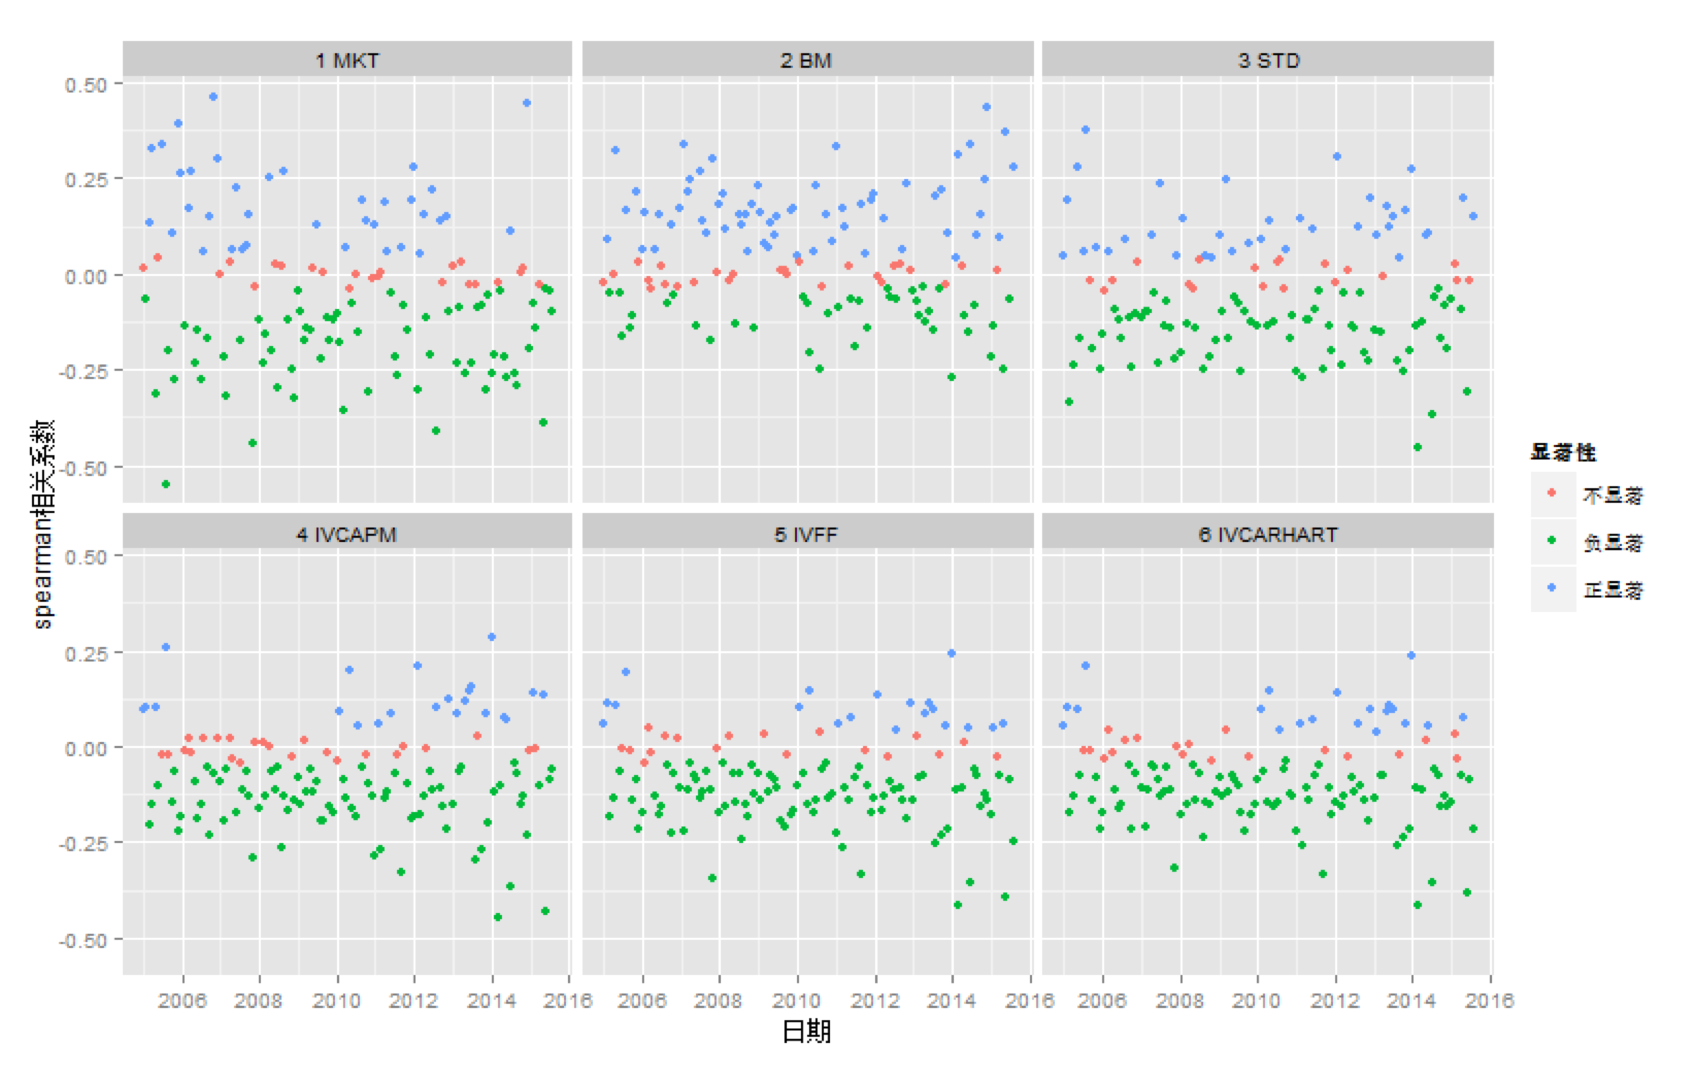
\includegraphics[scale=0.6]{figure/IC显著性.jpg}
\caption{IC序列}
\end{figure}

\begin{sdefinition}{单因子检验—分层检验}{}
在月末(调仓日),按照因子大小排序,将样本分为10组,这样我们认为在各组之间,因子值就没什么差别,然后在组内等权重构造投资组合,比较各组的表现,比如, \\
\boxgrey{年化收益,超额收益,信息比,月胜率,最大回撤等}。
\end{sdefinition}

\begin{figure}[htb]
\centering
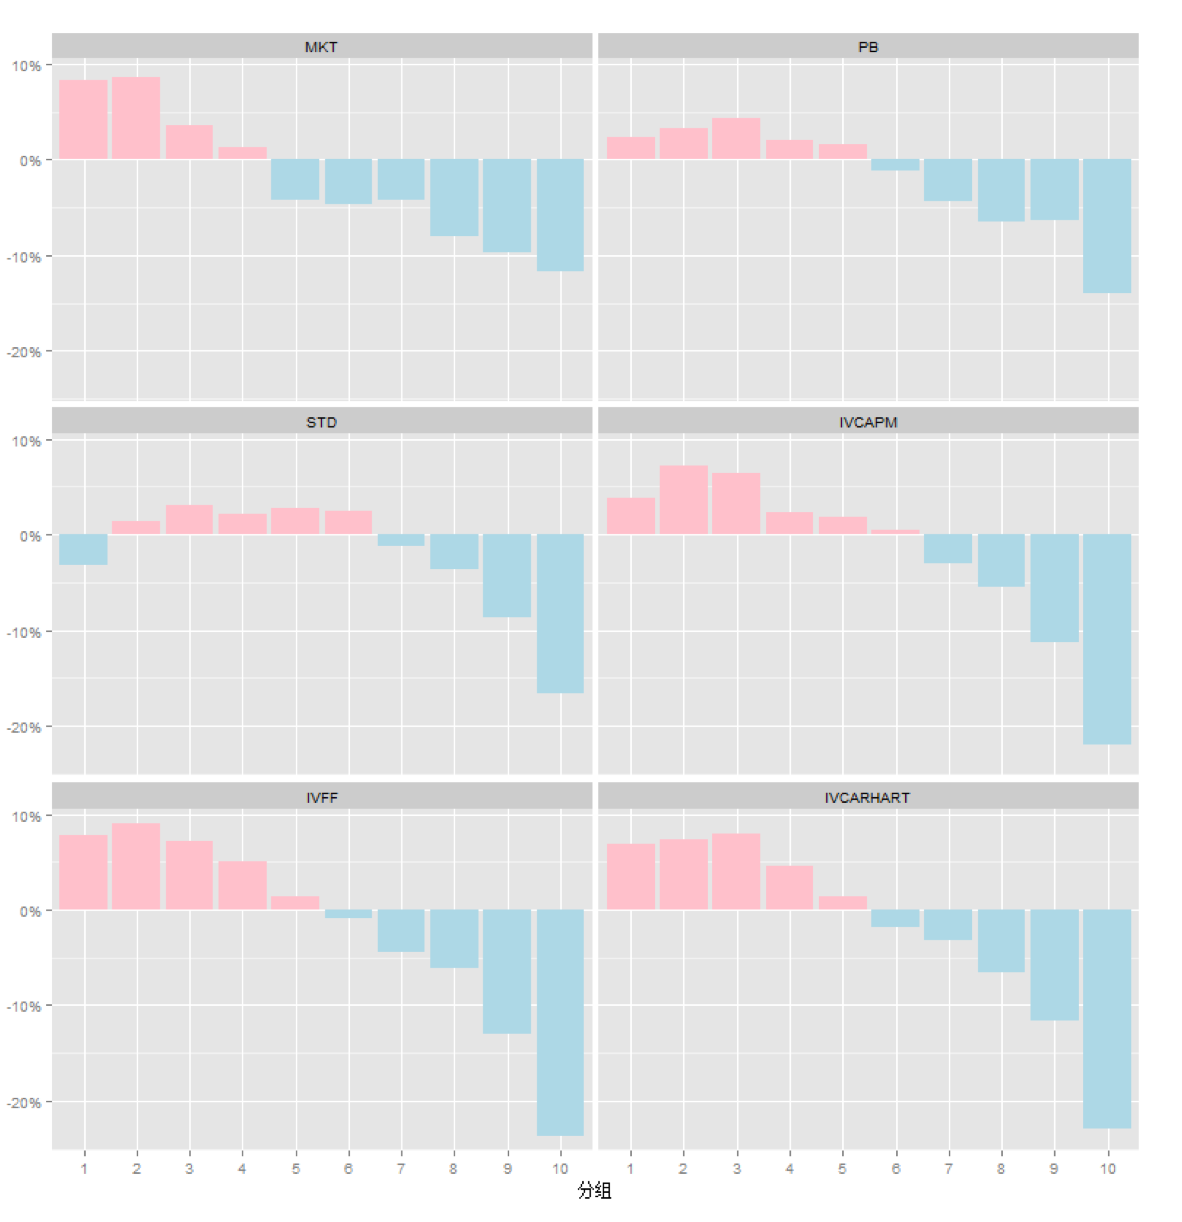
\includegraphics[scale=0.7]{figure/因子单调性.jpg}
\caption{比较理想的因子应当具有的效果(当然也有几个不理想的)}
\end{figure}

\begin{sdefinition}{单因子检验—多空组合}{}
做多优势组,做空劣势组构造投资组合,此时权重向量满足
$$
\omega^\prime \iota = 0.
$$
吗?
\end{sdefinition}
多空组合也是一个投资组合,我们可以利用之前的一些指标去评判。

\begin{sdefinition}{单因子检验—行业中性组合}{}
根据流通市值加权得到31个行业的权重向量$R^\prime \omega$,在不同行业间利用因子进行分组(等分为10组),各组之间等权重,把每个行业的第一组拿出来作为我们的优势组,依次类推。
\end{sdefinition}
\begin{sremark}{}{}
我对这个行业分层的理解就是呢,把因子对行业虚拟变量做了一个回归,然后取残差作为因子重新排序,效果应该差不多,试下推导。
\end{sremark}

\subsection{单因子检验II—剔除行业,风格后}
本节比上一节多了一个流程,也就是neutralize,为什么要Neutralize,因为我国A股市场具有明显的行业和市值效应,这也是很多因子的alpha来源。我们想要关注因子除去市值和行业后,还能够有产生超额收益的信息。
\begin{sdefinition}{单因子检验—风险调整IC}{}
	因子经过winsorize,standardize,neutralize后计算的IC值。
\end{sdefinition}


\subsection{因子间的相关性结构}
因子之间存在高相关性会对我们的模型产生灾难性的影响,所以我们需要剥离一个因子对另一个因子的影响,目前主要看到了分层+分组,将因子纳入回归,Fama-Macbeth这些办法,我们将逐一介绍。
值得注意的是,我们也关注因子的收益风险特征,所以也需要考察因子收益间的相关性。
\begin{sdefinition}{因子相关性—分层+分组}{}
可以用于剔除分层因子F对于分组因子对于收益率的影响
\end{sdefinition}
因子相关性分析可以让我们对超额收益归因,更好的构建多因子模型。
\begin{sremark}{}{}
假如我们有两个因子$F_1,F_2$, $F_1$分层,$F_2$分组后,构建多空组合,如果收益率变得不显著,那么$F_2$带来的超额收益主要源于$F_1$,就这么个逻辑,如果还是显著的,那么就可以认为$F_2$有除$F_1$之外的超额收益来源。
\end{sremark}



\begin{sdefinition}{因子相关性—因子收益率回归}{}
这里举一个例子吧,为什么这个部分和上个部分不同呢,做回归我们可以构造新的因子,而分层呢,不行(但可以加入固定效应?在换手率和市值的相关性分析中,我们发现经过市值分层后,低换手率股票仍然带有显著正向收益,因此将对数换手率,对对数流通市值回归后,残差项即可作为剔除市值影响后的换手率代理变量)
\end{sdefinition}
另外呢,为什么要用因子收益率呢?这里就涉及到了\boxgrey{多因子模型},做回归的目的在于,检验因子暴露是否显著以及检验alpha是否显著
\begin{sremark}{}{}
这个回归的因变量应该是股票收益率了,想想应该是面板,截面,时序中,哪个层面上的回归。
\end{sremark}
\begin{sremark}{}{}
然后还得注意,如果我们需要剥离因子的影响,这时候是用的因子值对因子值的回归。
\end{sremark}

\subsection{因子的IC的相关系数}
可以用于提高多因子模型的稳定程度 
\subsection{疑问}
作IC的时候,是用月末的因子和下个月的月均收益率呢,还是月末当天的收益率。答:一般是月末的因子和次月第一天的因子做相关系数,但也可以增加间隔的时间。
\section{alpha对冲}
为什么要叫alpha对冲呢?\\
在开始本章前,再次强调多因子模型的逻辑,首先是根据一套具有经济含义的投资逻辑,比如说购买具有相对低估值低高成长公司,而且这些公司没有被过度炒作。然后根据流程去挑选合适的因子合成为一个alpha,再通过一些约束,完成我们的优化问题。这里先给出优化的目标函数,
$$
\tcbhighmath{\max_{\omega} \ \alpha^\prime \omega - A\omega^\prime \Sigma \omega - \lambda \tau^\prime |\omega-\omega_0|}
$$
这样咱们就可以知道如何着手建模了。
\subsection{目标函数构建}
alpha模型,风险模型,成本模型,

\subsubsection{alpha模型}
在多因子择股量化投资流程中,alpha模型直接决定了投资组合能否获得稳健的超额收益。我认为构建alpha模型的要素不是从统计学意义上挑选因子,反而应当先构建一套符合经济学直觉的投资理论,比如我们想要挑选不那么被过度投机的股票,该过程称为\boxgrey{投资逻辑构建}。投资思路的确定缩小了因子的范围,然后我们再将这些因子筛选出来进行前文所述的检验,比如RANK IC,RANK IC的t统计量,IR,IC正负显著比例,多空组合的各项评判指标(收益率,波动率,夏普比,最大回撤等),条件允许的话还可以进行相关性分析等,最终挑选出少于10个优质因子值,我们称之为\boxred{alpha因子}。关于叫法来源,我觉得可能是这些因子很可能带来不错的alpha收益。\par
\begin{sremark}{}{}吴老师说 \\
有较为稳定的IC的因子叫做alpha因子,他们可以用于预测期望收益,因子我们常用alpha因子估计期望收益向量$\mu$. \\
如果只有一个因子,那么经过\boxred{处理}后直接作为$\mu$, 如果有多个因子,那么可以用下述整合办法去得到一个新的$\mu$。 
\end{sremark}

\begin{sremark}{}{}吴老师说 \\
需要值得注意的是,上述办法估计$\mu$,那么mu的含义已经不再是股票的期望收益,更多可以理解为借助alpha因子得到对这些股票的心理预期。
\end{sremark}

这就解释了为什么目标函数第一项是alpha。
接下来是利用这些alpha因子去构建选股策略,首先先把因子\boxgrey{处理}一下,winsorize,standardize,neutralize就行了,然后我们想办法把他们加总,这一步叫做\boxgrey{因子合成}。
我们可以采用下述办法进行加权,
\begin{sdefinition}{等权重合成}{}
现在不同类别的因子上分配相同的权重,然后在\boxgrey{同类因子}的内部再分配等权重。
\end{sdefinition}

\begin{sdefinition}{历史滚动IR加权}{}
\boxred{当各因子之间相关性较低时},我们可以使用这个办法,具体而言,先假设
$$
cv_t = \begin{bmatrix}
	cv(IC_{1,t}),\cdots,cv(IC_{k,t}).
\end{bmatrix}
$$
计算IC的cv时可以选用不同的滞后期数,最后我们因子的权重为
$$
\tcbhighmath{\omega_F = \frac{cv_t}{cv_t^\prime \iota}}
$$
\end{sdefinition}
啊,上边的有一些typo,应该是变异的倒数。
\begin{sdefinition}{历史面板数据进行回归}{}
被解释变量为股票的月度收益率,自变量是处理后的因子值,得到回归方程。利用最新一期的因子值更新数据,预测值作为"alpha"。
\end{sdefinition}


当然,在\boxred{研报八—动态情景的多因子Alpha模型}中会介绍更复杂的加权办法,当然我们这里得到的叫因子综合得分,究竟是不是这里的alpha,还有待而论。

\begin{sdefinition}{动态情景+历史滚动IR}{}
	研报八里边那个,相对于一般的历史滚动,加入了情景因子。但我有点没看明白他怎么给情景因子赋的权重。
\end{sdefinition}

\begin{sremark}{}{}
当然,如果对于既定目的下,经济学含义特别明显的因子,我们还有其它的加权方法,比如加总Copula,这个说法不太严谨,但我自己能明白是啥意思,实在明白不了?那想想交易热度怎么构建的吧。
\end{sremark}

\subsubsection{风险模型}
我目前对于风险模型的理解是,目标函数中的第二项,控制投资组合的风险。而风险有多种度量方式,比如协方差矩阵,当然,如果直接用协方差矩阵的话,一个是咱们的这个T必须大于股票数量N,第二呢,可能存在一些噪声,所以我们也有一系列改进方案,当然,还是按照流程来
\begin{sdefinition}{风险模型-协方差矩阵}{}
	我们利用协方差矩阵刻画整体风险,具体计算办法为:
$$
S = \frac{1}{T}X^\prime(I-\frac{1}{n}\iota \iota^\prime)X.
$$
\end{sdefinition}
\begin{sremark}{}{}
	有一些问题,比如我们采用月度调仓,股票池中有2000只股票,此时需要时序上大于2000次观测,这可行吗?所以改进一下
\end{sremark}

\begin{sdefinition}{风险模型-因子模型}{}
$$
S_t = B_tF_tB_t^\prime + E 
$$
其中B为因子暴露矩阵
\end{sdefinition}
利用$BFB^\prime$对风险进行衡量。
\begin{sremark}{}{}
因子模型有,基本面因子模型,宏观因子模型,统计因子模型(把主成分作为因子),这里可以来一个详细推导。
\end{sremark}

\begin{sdefinition}{风险模型-协方差矩阵压缩估计量}{}
$$
\Sigma_{shrink} = (1-\beta)F + \beta S
$$
\end{sdefinition}
\begin{sremark}{}{}
会不会有Bayes信度模型。
\end{sremark}


\subsubsection{成本模型}
目前先不看,目前用到的主要是常数交易费用。

\subsection{优化问题}
\subsubsection{Basic Form}
假设我们通过因子检验,合成,已经通过加权,构造了因子向量alpha(在一个时间截面上,一只股票对应一个alpha),假定股票池有n只股票,我们的目标是在控制风险和成本的情况下最大化alpha(为什么不是最大化收益,我猜测是收益率是随机游走,基本不存在自相关性,现在收益高不代表未来收益高,所以最大化收益向量不如最大化我们这里的alpha,至少这里的alpha都是比较能预测未来收益率的)
$$
\tcbhighmath{\max_{\omega} \ \alpha^\prime \omega - A\omega^\prime \Sigma \omega - \lambda \tau^\prime |\omega-\omega_0|}
$$
s.t.
\begin{eqnarray*}
	& &R^\prime \omega = R^\prime \omega_{\text{bench}} \\
	& &\omega^\prime \iota = 1 \\
	& & 0 \leq \omega_i \leq \min(maxposition, \omega_{0,i}+maxtradesize_i/booksize_i) 
\end{eqnarray*}
\par
值得注意的是,$\alpha$应该是合成的alpha因子,A代表风险厌恶系数,$\lambda$用于控制交易成本。
关于目标函数的解读,首先是要最大化alpha因子,也就是目标函数的第一项,第二项用于控制投资组合的风险,最后一项绝对值是逐项运算,用于控制成本。\par
关于约束条件的解读,R是一个$31\times300$的矩阵,每一列之和为1,用于存储股票的行业信息。因此我们的第一个条件含义在于,投资组合中资金分配在一个行业的比例,应该等于行业内动态市值加权的占比。第二,第三个条件比较容易理解。一个变种是加入\boxgrey{显性跟踪误差约束条件}
$$
\tcbhighmath{\max_{w} \quad \alpha^{\prime} w-\lambda \tau^{\prime}|w-w_0|}
$$
s.t.
$$
\tcbhighmath{
\begin{aligned}
&\mathrm{R}^{\prime} w=R^{\prime} w_{\text {bench}} \\
&\left(w-w_{\text {bench }}\right)^{\prime} \Sigma\left(w-w_{\text {bench }}\right) \leq \frac{T E^2}{252} \\
&\omega^{\prime}\iota =1 \\
&0 \leq w_i \leq \min \left(\text { maxposition, } w_{0, i}+\text {maxtradesize}_i / \text {booksize}_t\right)
\end{aligned}}
$$
\begin{sremark}{}{}
对于新加的这个约束,我的理解是相当于控制一个多空组合的风险,因为$(\omega-\omega_{bench})^\prime \iota =0$
\end{sremark}



规划求解问题:
\subsection{归因分析}

\section{调仓频率}
调仓频率和因子的信息衰减速度需要做一个匹配,以充分利用因子的信息。
\section{一些有待解决的问题}
\subsection{行业中性化的相关问题}
我们在优化问题中提到了,
$$
R^\prime\omega = R^\prime \omega_{bench}
$$
这个条件和行业中性化有些像。所以再仔细想想呢?

\section{因子挖掘}



\section{因子挖掘—交易行为类}
在构造一个因子前,我们需要去说明一套能赚钱的投资理论,然后结合理论去寻找量化指标。
\subsection{投资逻辑}
投资逻辑,A股市场投机氛围浓厚,规律是被投机的股票后期大概率跌,而相对正常的股票,反而会涨,所以我们的逻辑是卖投机程度高的,买投机程度不足的。逻辑虽然简单,但投机程度无法观测,我们需要去构造能够衡量投机程度的指标。
\subsection{指标构建}
过度投机的股票会有,\boxgrey{高波动性,风格独立,价格时滞,高换手}的特点,所以我们分别采用下述四个指标对其进行衡量\\
特质波动率 \\
我们用特质波动率来衡量个股的波动程度,特质波动率实质是条件方差,所以我们用条件方差的均值进行刻画。
$$
\tcbhighmath{\text{特质波动率}^2 = \frac{SSR_{Fama}}{n}}
$$
被投机的股票多空分歧大,进而展现出大的波动。\\
特异度 \\ 
被过度投机的股票会过分利用自身信息,忽视市场规律,从而我们的$Fama-French$模型对股价的解释力度较差,这说明$R^2$较低. 因此我们定义
$$
\tcbhighmath{IVR = \frac{SSR}{SST} = \frac{\text{特质方差}}{\text{总方差}}}
$$
价格时滞 \\
过度投机的股票不能及时反应价格信息,但这并不意味着过去的信息就有用,所以我觉得讨论这个指标纯粹是浪费时间。\\
高换手\\
过度投机的股票换手率较高,这个很容易理解,但市值和换手率相关度较高,所以我们先取对数(让数据服从正态),然后将对数换手率关于对数市值作一个正交分解,将残差作为\boxgrey{市值调整的收益率}
\subsection{交易热度I}
经过相关性分析,我们发现特异度和市值调整换手能够包含其他交易行为类指标的所有信息,我们利用加总分位数的方式合成了一个新的因子,叫做交易热度
$$ 
\text{BehaviorIndex}_{i, t}=\frac{1}{2}\left[Q\left(\operatorname{IVR}_{i, t}\right)+Q\left( adjTurnover_{i, t}\right)\right]
$$
其中,BehaviorIndex $x_{i, t}$ 为股票 $\mathrm{i}$ 在时刻 $\mathrm{t}$ 的交易热度,IVR $R_{i, t}$ 为股票 $\mathrm{i}$ 在时刻 $\mathrm{t}$ 的特异度, adjTurnover $_{i, t}$ 为股票 $\mathrm{i}$ 在时刻 $\mathrm{t}$ 的市值调整换手。 $Q\left(I_{i, t}\right)$ 表示股票 $\mathrm{i}$ 的指标 $I_{i, t}$ 在时刻 $\mathrm{t}$ 样本空间内 所有股票中所对应的分位数 (累计分布概率)。
交易热度在0,1中取值,而且我们取分位数的操作(其实也是嵌入广义逆)是一个单调变换,\boxgrey{不会改变秩相关系数},因此可以预计到,他基本和对数流通市值不相关。
\begin{sremark}{}{}
这个Q(X),代表X的分位数,其实差不多就是F(X), 其中F是经验累积分布函数,所以差不多Q(X)就可以看作一个均匀随机变量(的观测)。	
\end{sremark}
\begin{figure}[htb]
	\centering
	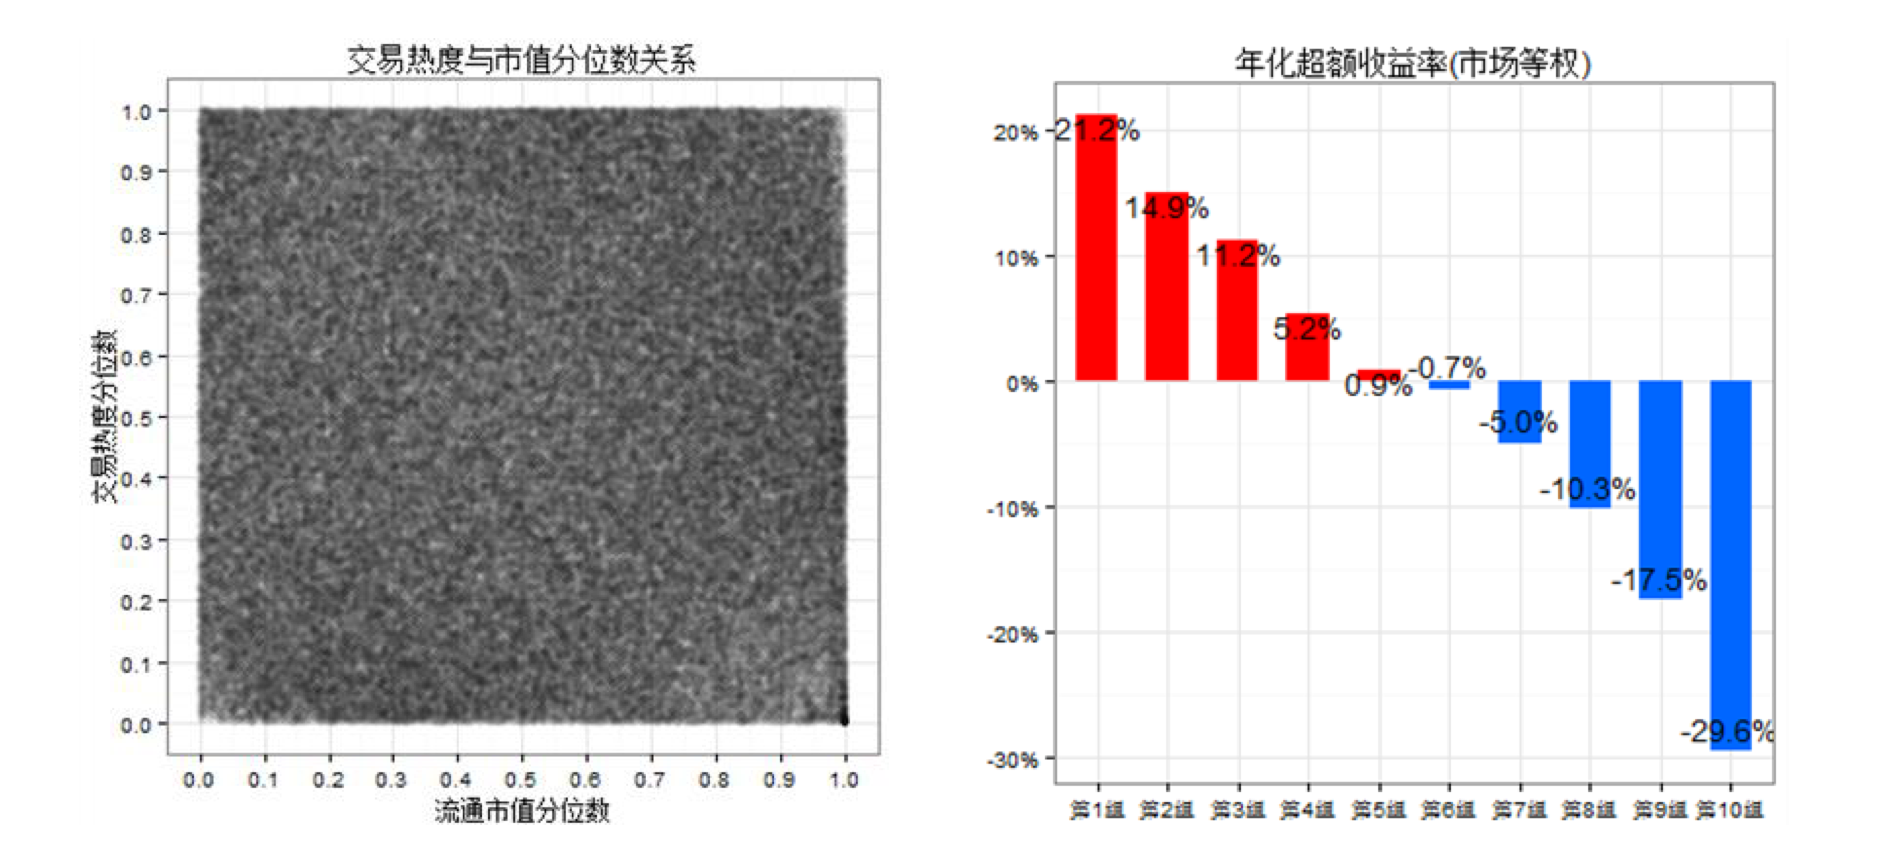
\includegraphics[scale=0.5]{figure/交易热度1.pic.jpg}
	\caption{交易热度和流通市值的关系以及分组表现(看起来像独立copula)}
\end{figure}

\begin{figure}[htb]
	\centering
	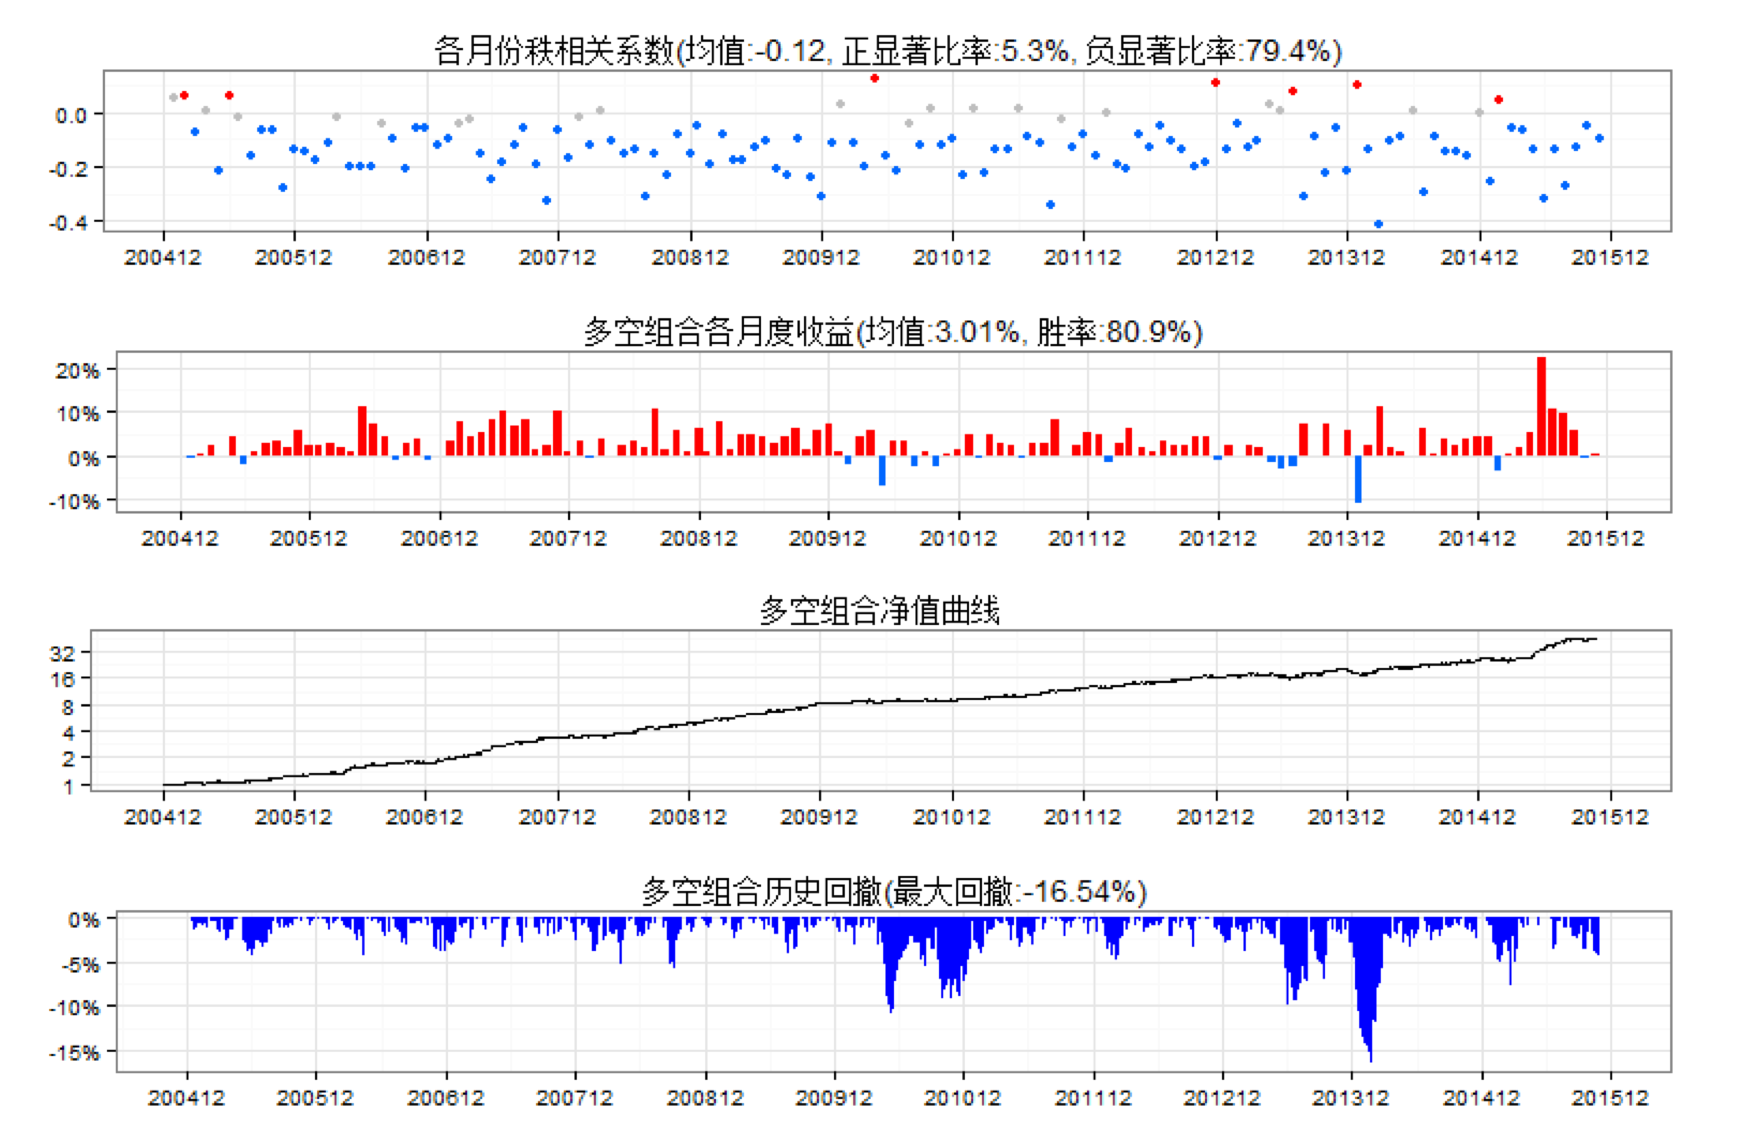
\includegraphics[scale=0.5]{figure/交易热度1历史表现.png}
	\caption{交易热度历史表现}
\end{figure}

\subsection{交易热度II}
我们在下一节定义了一个价差偏移度,不同于特异度和市值调整换手,价差偏移度直接从股票价格与其相似股票的偏离程度出发,以衡量股票的投机程度。由于三个指标有明显的超额收益,而且信息来源相对独立,所以综合起来更新交易热度,
$$ 
\text{BehaviorIndex}_{i, t}=\frac{1}{3}\left[Q\left(\operatorname{IVR}_{i, t}\right)+Q\left( adjTurnover_{i, t}\right)+Q(SpreadBias_{i,t})\right]
$$
可以发现交易热度市值是3个均匀随机变量之和,交易热度越高,股票相对高估,后期预期收益率较低。

\begin{figure}[htb]
	\centering
	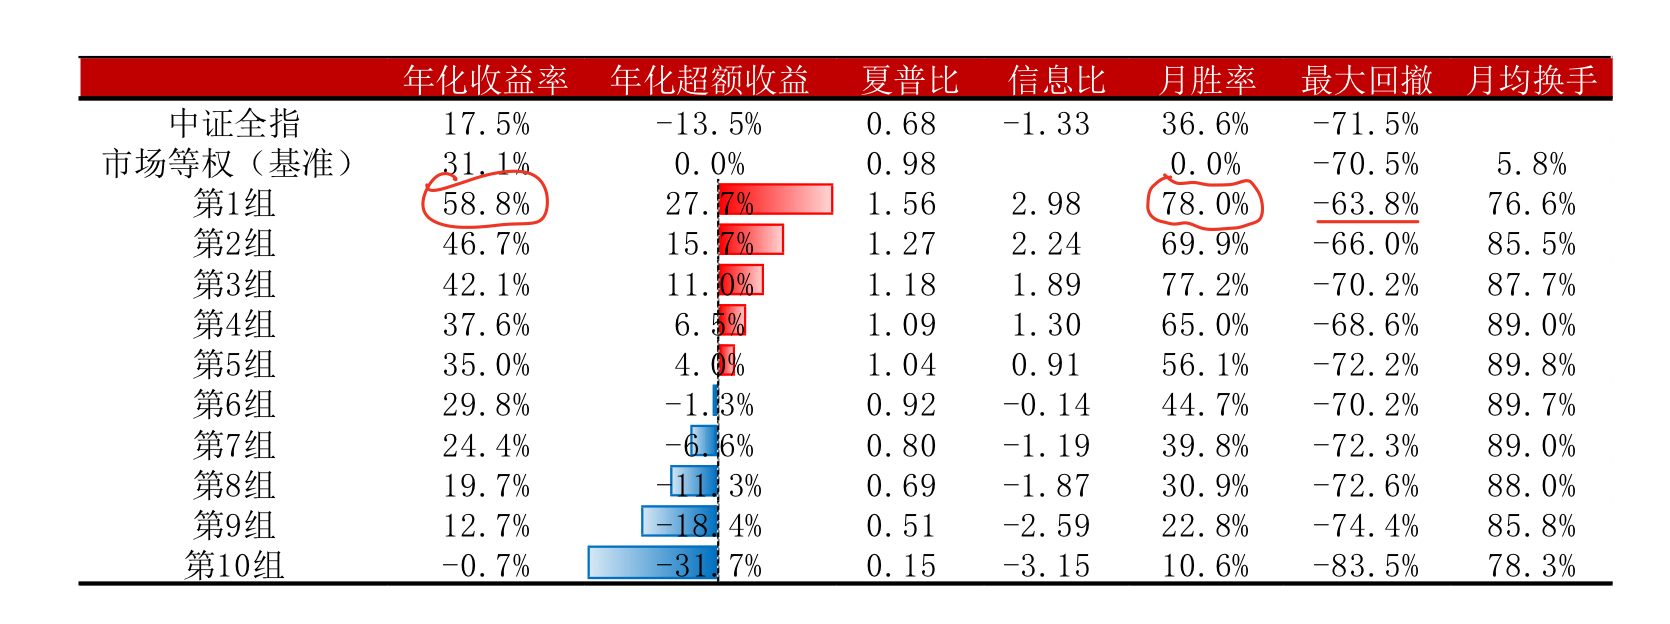
\includegraphics[scale=0.5]{figure/交易热度3因素_历史表现.png}
	\caption{交易热度3因素,历史表现}
\end{figure}


\section{因子挖掘—价差偏移度}
我们利用了特异度和市值调整换手这两个交易行为类指标去衡量个股被投机的程度。但他们直接没有从股票的价格考虑股票被相对高估低的情况。
\subsection{投资逻辑}
股票的涨跌以概念,板块的方式\boxred{轮动炒作}。事实上,某一板块大部分股票都涨时,其它没涨的股票就有补涨的需求,反之也成立。因此,当类别A的某只股票表现弱于其相似的股票时,买入则可能获得超额收益。
\subsection{指标构建}
借助\boxgrey{统计讨论}的思想,我们提出\boxgrey{价差偏移度},试图捕捉股票相对同类型股票的相对高低估程度。
\begin{sdefinition}{股票的距离}{}
$$
d(S_i,S_j) = 1 - corr(S_i\text{的过去250交易的日涨跌幅度},S_j\text{的过去250交易的日涨跌幅度}) 
$$
\end{sdefinition}
当然,上边的这个距离不满足三角不等式(满足吗?),从而并不满足距离的公理化定义,但对于我们的问题,这个距离已经够用了。

\begin{sconclude}{价差偏移度的构建流程}{}
1. 固定股票i,提取i距离最近(d(i,j)最小的10个j)的10只股票,等权重构成参考价格(ref)\\
2. 定义对数价差 $$ \tcbhighmath{\text{PriceSpread}_{i,t}=\ln{S_{i,t}}-\ln{ref_{i,t}}}$$ 
3. 计算过去60日对数价差的Z-score(时间序列上),作为价差偏移度.

\end{sconclude}
\begin{sremark}{}{}
价差偏移度是一个相对意义上的反转因子,价差偏移度低,股票跑输组合,估值较低,未来会涨,买入将获得超额收益,反之成立。 值得注意的是,上述成立的一个必要条件是,股票基本面没有发生重大变换。
\end{sremark}


\subsection{因子检验}
\subsubsection{分组}
\begin{figure}[htb]
	\centering
	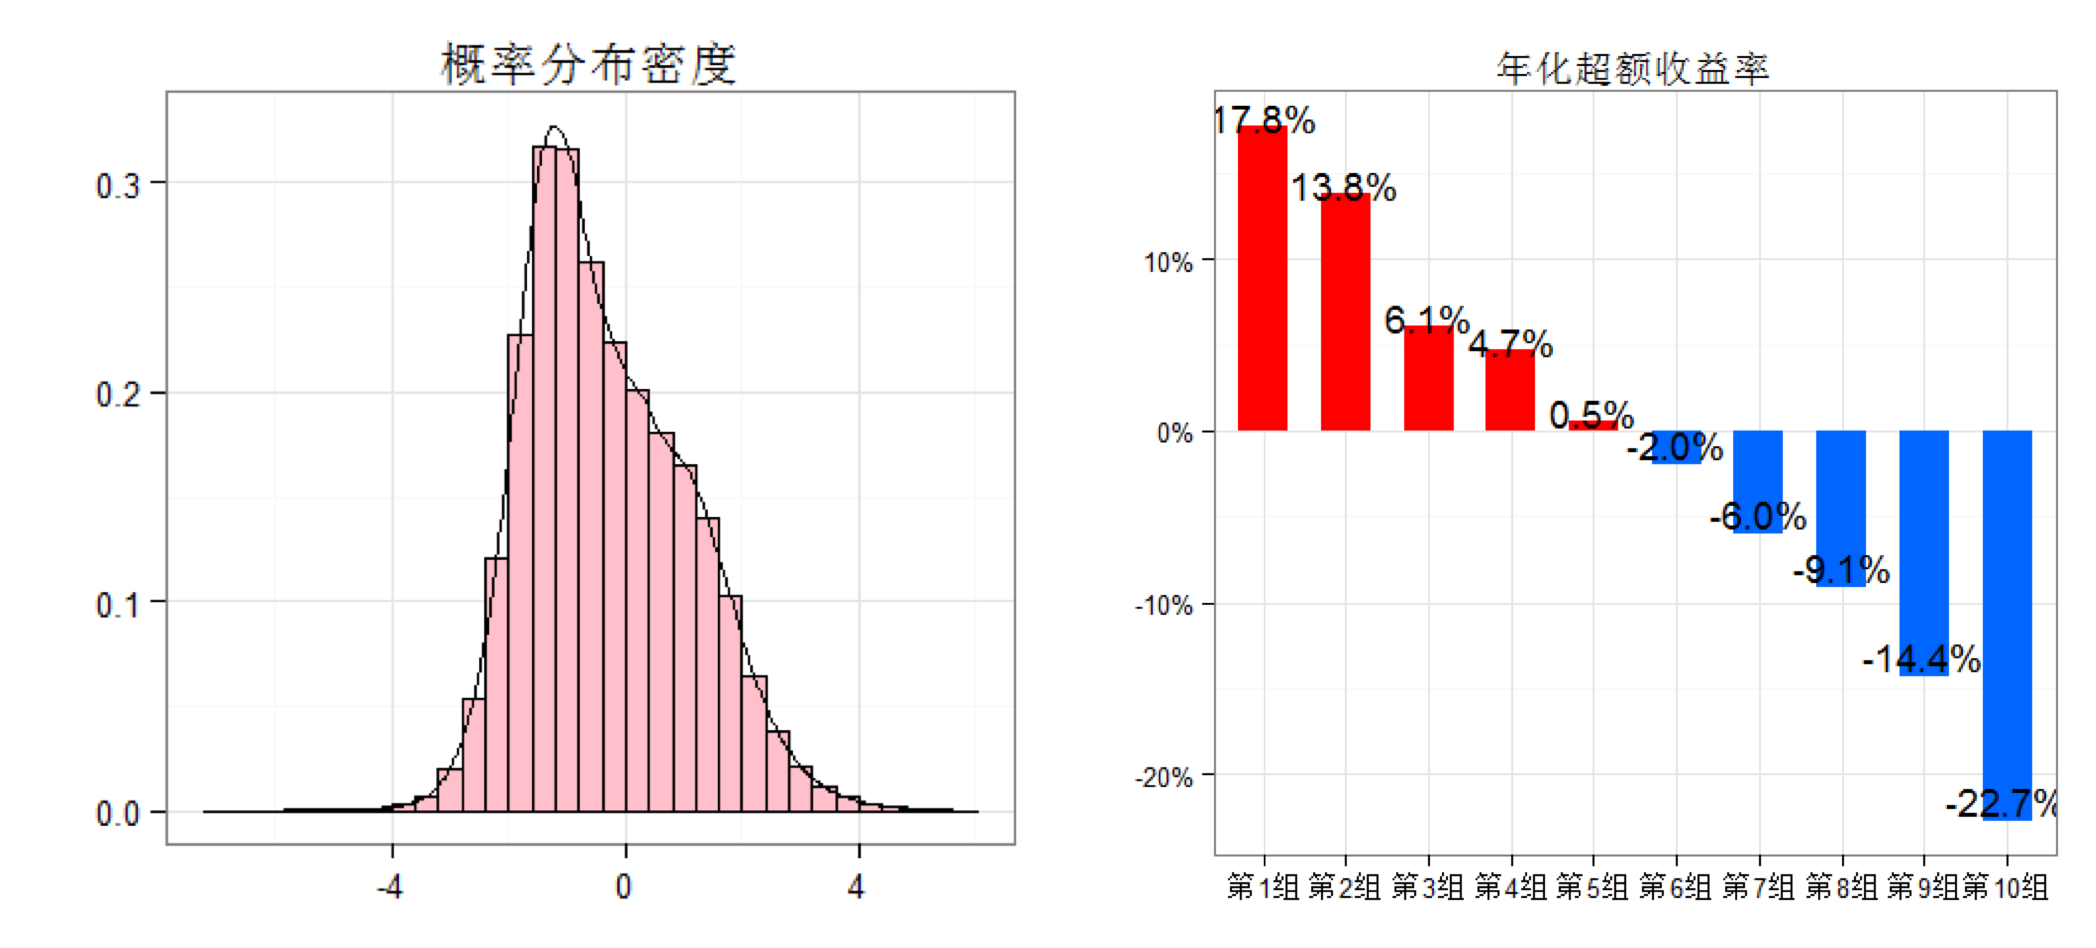
\includegraphics[scale=0.45]{figure/价差偏移度_分组.png}
	\caption{价差偏移度的分组收益}
\end{figure}
满足单调性, 然后分布呢,不知道怎么形容。
看看历史IC和多空组合的历史表现吧,
\begin{figure}[htb]
	\centering
	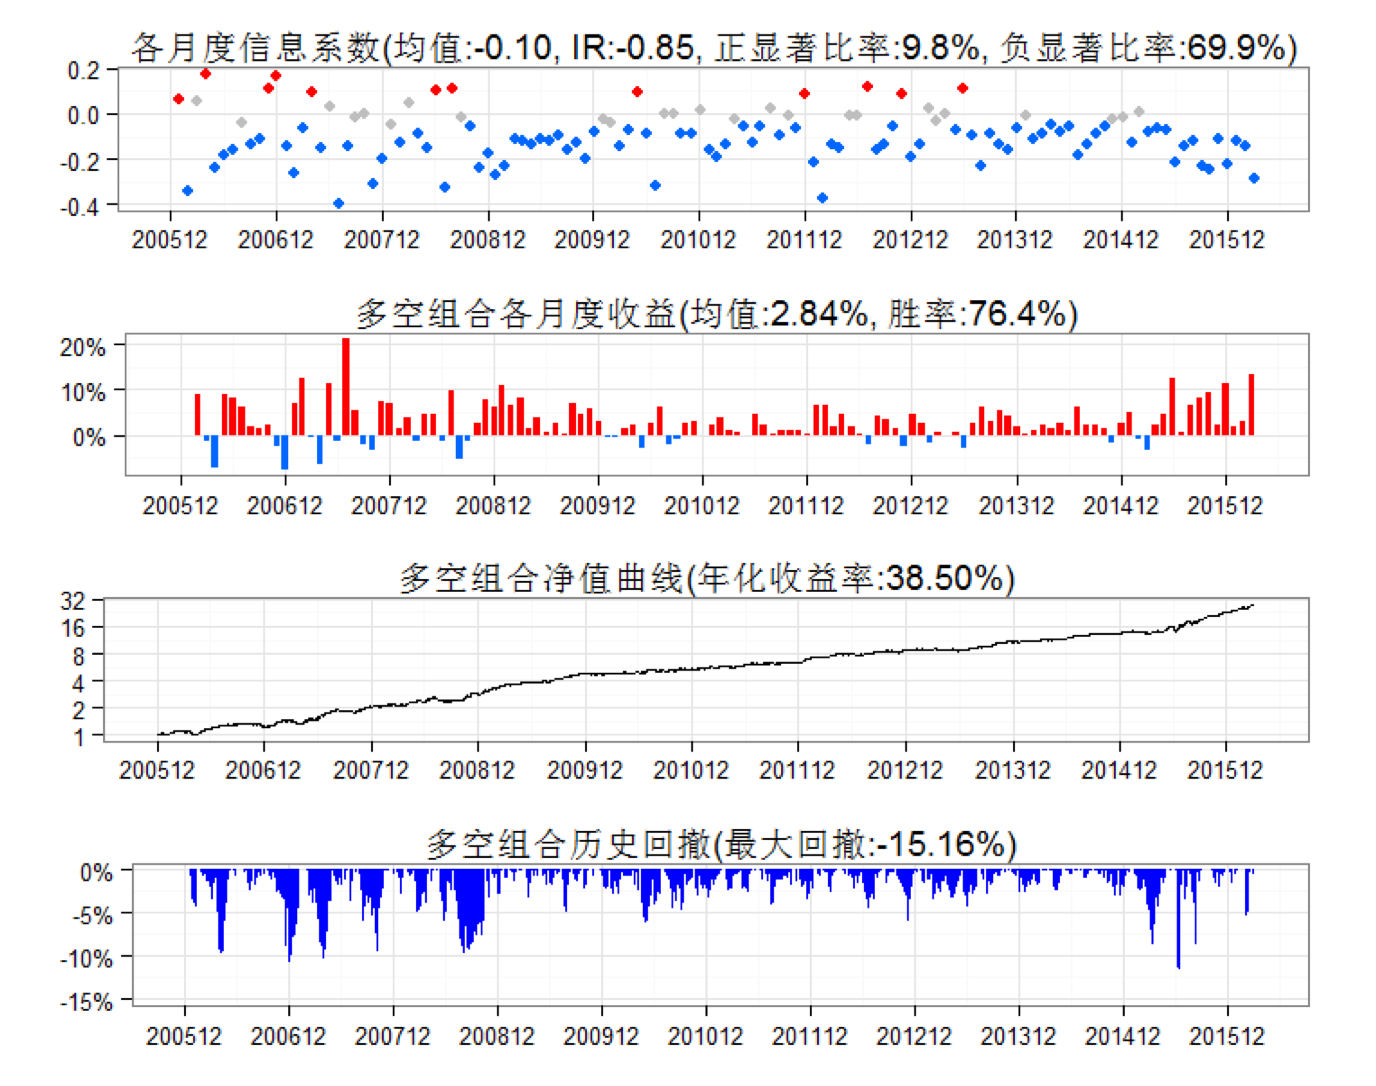
\includegraphics[scale=0.7]{figure/价差偏离度_历史表现.png}
	\caption{价差偏移度的历史表现}
\end{figure}
\subsubsection{相关性分析}
价差偏移度是一个相对的反转因子,所以和1个月反转,3个月反转有相关性,然后我们这里利用,
\boxgrey{分层+分组}构建多空组合,\boxgrey{Fama-Machbeth}对收益来源进行归因。


\section{因子挖掘—日内残差高阶矩}


\section{因子—波动率}
我们提到资产的波动率时,是指价格的标准差,还是收益的标准差。
波动率可以分为实际波动率, 历史波动率, 隐含波动率,预测波动率等。





\section{研报阅读一}
\cite{ori1}
\subsection{单因子有效性检验}
量化选股主要涉及到两个核心的问题。第一,如何 选出有逻辑意义并且能够有效的区分个股的因子,使得因子值对于个股未来收益有一定的预测能力。 第二,影响市场的因子众多,且市场风格并非一成不变,我们如何构建一个能够适应市场变化的多 因子模型,筛选出大概率能够战胜市场的股票组合
\begin{sconclude}{}{}
\begin{itemize}
	\item 
	\item 市值因子,反转因子,换手率指标,各类业绩增速指标和估值指标表现较好
	\item 资产负债率,周转天数,ROE,ROA,销售利润对股价有一定的预测性
\end{itemize}
\end{sconclude}


\subsection{单因子检验}
我们的目标在于检验因子与未来收益率是否存在显著相关性。主要流程是,按照每一期指标值大小对股票分组,这样各组的指标可以看作一致,然后比较各组的表现,比如\boxgrey{累计收益,信息比率,最大回撤,胜率等}, \boxred{单调性越强,优势组的胜率越高}。
\subsubsection{OLS v.s. Robust}
Robust能够容忍异常值
\subsubsection{整体回归 v.s. 按月度回归}
按月度回归的好处:减少样本量(样本量过大会导致相关系数显著),有利于观察指标的历史变化情况,比如正负月份的具体比例,因子的持续周期和反转频率
\subsubsection{相关系数的度量}
Pearson,Spearman rho, kendall tau对比,后面俩可以度量非线性关系,但随时了边缘分布的信息,\boxred{经验法则是Spearman rho的显著比例高于Pearson rho}。

\subsubsection{是否应当行业中性化}
基本面因子,如\boxgrey{PB,资产周转率,市值},存在\boxred{行业固定效应},所以全市场分组不合理。,行业中性化相当于,我们在每个行业按照PB进行分组,在根据流通市值加权,这样就可以认为每组的不存在行业固定效应了。
\subsubsection{同向显著比例,状态切换比例}
用当月因子值与次月收益率算出来的回归系数,可能随时时间发生改变,实际预测的时候怎么办呢?\\
1. 选择正负比例中较高的那个, 2. 如果因子的特性延续性较好,则可以最近一期的数据情况对下一期进行预测。

\subsection{结果展示及业界通用做法}
\begin{sconclude}{}{}
	\begin{itemize}
		\item 衡量因子是否显著:秩相关系数正/负比例至少一项大于0.35, 或者之和大于0.6
		\item 是否行业中性化:行业内分组的优胜组年化超额收益大于全市场分组
		\item 因子稳定度的衡量:1.同向显著次数大于状态切换次数,说明因子有一定趋势 2. 当同向显著的比例大于 max(正显著相关,负显著相关),则在后续的多因子模型建立中,动态的决定指标的参数可能胜率更

	\end{itemize}
\end{sconclude}
一些疑问是, \boxred{本月因子值与下月收益率做回归,但问题是数据的长度可能不匹配}, 而且对应规则如何呢?是当前月第一天对应次月第一天吗? 还有就是所有因子每天都有数据吗?会不会有某些因为长时间保持不变呢?或者说,我们做的是截面上的回归,那这和样本量有什么关系呢?\par
是否只有单调性好的指标才是好的因子?并不是,某些因子的特性,或者要达到一定阈值后因子的效果才会体现出来。

\section{研报阅读二—特质波动率}
\subsection{现象及结论}
低特质波动率,未来预期收益更高。
首先是特质波动率,严格定义一下,在因子模型中,我们认为个股i的超额收益率为
\begin{stheorem}{方差分解}{}
$$
R_i = \alpha + \inner{B}{F} + \epsilon_i
$$
$$
\tcbhighmath{Var(R_i)=Var(E(R_i|F))+E(Var(R_i|F))}
$$
\end{stheorem}
我们认为$Var(R_i|F)$就是$R_i$的特异风险的平方。

\begin{sconclude}{}{}
\vspace{-.4mm}
\begin{itemize}
	\item FF三因子模型残差的波动率能更好捕捉股票的特质风险,记作IVFF.(好体现在哪里)
	\item 特质风险与未来截面收益率存在负相关关系,IVFF预测能力最强
	\item 
\end{itemize}
\end{sconclude}


\section{研报阅读三—交易行为与股票收益}
\begin{sconclude}{}{}
\begin{itemize}
	\item 投机程度弱的股票未来大概率涨,所以应当买入
	\item 通过交易行为指标度量投机程度,具体有: \\ \boxgrey{特征波动率,特异度,价格时滞,市值调整换手}
	\item 这些交易行为类指标均表现出较强的收益预测能力
	\item 特异度和市值调整换手在控制其他交易行为类指标后还能带来超额收益。
\end{itemize} 
\end{sconclude}

\subsection{交易行为类指标}
过度投机的股票会有,\boxgrey{高波动性,风格独立,价格时滞,高换手}的特点。
\subsubsection{特质波动率}
我们用特质波动率来衡量个股的波动程度,特质波动率实质是条件方差,所以我们用条件方差的均值进行刻画。
$$
\tcbhighmath{\text{特质波动率}^2 = \frac{SSR_{Fama}}{n}}
$$
被投机的股票多空分歧大,进而展现出大的波动。

\subsubsection{特异度}
被过度投机的股票会过分利用自身信息,忽视市场规律,从而我们的$Fama-French$模型对股价的解释力度较差,这说明$R^2$较低. 因此我们定义
$$
\tcbhighmath{IVR = \frac{SSR}{SST} = \frac{\text{特质方差}}{\text{总方差}}}
$$
\subsubsection{价格时滞}
过度投机的股票不能及时反应价格信息,但这并不意味着过去的信息就有用,所以我觉得讨论这个指标纯粹是浪费时间。
\subsubsection{高换手}
过度投机的股票换手率较高,这个很容易理解,但市值和换手率相关度较高,所以我们先取对数(让数据服从正态),然后将对数换手率关于对数市值作一个正交分解,将残差作为\boxgrey{市值调整的收益率}


\section{研报阅读八—动态情景多因子Alpha模型}
\subsection{Alpha模型的构建}
什么是alpha模型?alpha模型的最终目标在于给股票未来收益率排序,核心是因子的挑选和不同因子间的权重配比。动态情景alpha模型,Dynamic Contextual Alpha(DCA),
\section{研报阅读九—日内残差高阶矩与股票收益}
高频数据,分笔数据(tick),快照数据(quote),分钟数据,资金流量数据等。
日内价格行为特征和股票未来收益率之间的关系

\section{研报—波动率}




\bibliographystyle{siam}
\bibliography{ref.bib}
%\bibliographystyle{osajnl}
\end{document}


